%\documentclass[12pt,letterpaper,oneside,final]{memoir}
\documentclass[letterpaper]{polythesis}
\usepackage[medium]{titlesec}
\usepackage{calc}
\usepackage[subfigure]{ccaption}
\usepackage{subfigure}
\usepackage{enumerate}
\usepackage{tabularx}
\usepackage{algorithm2e}
\usepackage{url, cite, graphicx, amsmath, amsfonts, amsthm, float}
%\usepackage{url, cite, graphicx, algorithmic, amsmath, amsfonts, amsthm}
%\usepackage[chapter]{algorithm}
\usepackage{multirow}
\usepackage[titletoc]{appendix}
\usepackage{pifont}
\usepackage{color}
\usepackage{soul}
\usepackage{pythonhighlight}
\newtheorem{condition}{Condition}[section]
\newtheorem{definition}{Definition}[section]
\newtheorem{theorem}{Theorem}[section]
\newtheorem{lemma}[theorem]{Lemma}
\newtheorem{cor}[theorem]{Corollary}
\newtheorem{corollary}[theorem]{Corollary}
\newtheorem{claim}[theorem]{Claim}
\newtheorem{fact}[theorem]{Fact}
\newtheorem{example}[section]{Example}
\newtheorem{note}{Note}[section]

%% Some trickery to be able to add stuff in before the first chapter.
\def\nonumchapter#1{%
    \chapter*{#1}
    \addcontentsline{toc}{chapter}{#1}}

\def\prefacesection#1{%
    \chapter*{#1}
    \addcontentsline{toc}{chapter}{#1}}

\def\afterpreface{\newpage
    \pagenumbering{arabic}
    \typeout{Dalthesis preface pages completed.}
    }

%%%%%%%%%%%%%%%%%% for pangolin %%%%%%%%%%%%%

\newcommand{\techreport}[1]{}
\newcommand{\submission}[1]{#1}
\newcommand{\bda}	{\begin{eqnarray*}}
\newcommand{\eda}	{\end{eqnarray*}}
\newcommand{\bdalign}	{\begin{align*}}
\newcommand{\edalign}	{\end{align*}}
\newcommand{\define}	{\equiv}
\DeclareMathOperator*{\argmin}{arg\,min}


\newcommand{\be}{\begin{equation}}
\newcommand{\ee}{\end{equation}}
\newcommand {\beq}{\begin{equation}}
\newcommand {\eeq}{\end{equation}}
\newcommand {\bear}{\begin{eqnarray}}
\newcommand {\eear}{\end{eqnarray}}
\newcommand {\bearn}{\begin{eqnarray*}}
\newcommand {\eearn}{\end{eqnarray*}}
\newcommand {\barr}{\begin{array}}
\newcommand {\earr}{\end{array}}
\newcommand {\done} {\hfill\quad\vrule height4pt WIDTH4PT}
\def\cee#1#2{\left(\barr{c} #1\\ #2 \earr \right)}
\def\tA{\tilde{A}}
\def\tL{\tilde{L}}
\def\tM{\tilde{M}}
\def\real{{\rm I\!R}}
\def\cS{{\cal S}}
\def\cF{{\cal F}}
\def\hT{\hat{T}}
\def\naive{na\"{\i}ve}


\newcommand{\myvec}[1]{\mathbf{#1}}
\newcommand{\mymatrix}[1]{\mathbf #1}
\newcommand{\rank}{\mathrm{rank}}
\newcommand{\myspan}{\mathrm{span}}
\newcommand{\mynull}{\mathrm{null}}
\newcommand{\mysize}{\mathrm{size}}
\newcommand{\myenqueue}{\mathrm{enqueue}}
\newcommand{\mypop}{\mathrm{dequeue}}
\newcommand{\mymatching}{\mathrm{matching}}

%%%%%%%%%%%%%%%%%% for pangolin end %%%%%%%%%%%%%

\usepackage[babel=once,english=american,autostyle=tryonce,strict=true]{csquotes}

\usepackage[final]{hyperref}%?%hyperfootnotes=false
\hypersetup{%bookmarks=false,        % show bookmarks bar?
    unicode=true,           % non-Latin characters in Acrobat’s bookmarks
    pdftoolbar=true,        % show Acrobat’s toolbar?
    pdfmenubar=true,        % show Acrobat’s menu?
    pdffitwindow=false,     % window fit to page when opened
    pdfstartview={FitH},    % fits the width of the page to the window
    pdftitle={PhD Thesis},
    pdfauthor={Author Name},     % author name goes here
    pdfsubject={PhD Thesis},   % subject of the document
    pdfcreator={Author Name},   % creator of the document
    pdfproducer={Author Name}, % producer of the document
    pdfkeywords={}, % list of keywords
    pdfnewwindow=true,      % links in new window
    colorlinks=true,       % false: boxed links; true: colored links
    linkcolor=black,          % color of internal links
    citecolor=black,        % color of links to bibliography
    filecolor=black,      % color of file links
    urlcolor=black           % color of external links
}


%\usepackage{svg}
%--------From BRAIN --------%
\usepackage{tabularx}
\RequirePackage[english=usenglishmax]{hyphsubst}
\usepackage{calc}
\usepackage{multirow}

\usepackage{tabularx,ragged2e,booktabs}
\newcolumntype{C}[1]{>{\Centering}m{#1}}
\renewcommand{\arraystretch}{1.3}
%\usepackage{dblfloatfix}

\begin{document}
%\fussy
%\hyphenpenalty=5000   %1000 default=?
%\tolerance=1000        %1000 %200= default
%\setlength{\emergencystretch}{3em}
%\midsloppy
\fussy
\vbadness=10000 % badness above which bad vboxes are shown. (Default = 10000?)
\frontmatter
\hyphenation{}

\doublespacing

\begin{center}

\thispagestyle{empty}
{\Huge \bfseries Face Recognition with Eigenfaces}


\vspace{20mm}
by\\
\vspace{10mm}
Haonan Wu\\
N18859539\\
\vspace{30mm}
New York University\\
Dec, 2017
\end{center}
\vspace{35mm}
\begin{flushright}
{\rule[0pt]{45mm}{0.1mm}}\\ %rule[raise-height]{width}{height} * raise-height specifies how high to raise the rule (optional) * width specifies the length of the rule (mandatory) * height specifies the height of the rule (mandatory)

E.D Wong
\end{flushright}

\newpage

\thispagestyle{empty}

\begin{center} Copyright © 2019 Haonan Wu \end{center}

\newpage
\renewcommand{\contentsname}{Table of Contents}
\tableofcontents

\afterpreface

\mainmatter

\doublespacing
\mainmatter
\clearpage
\cleardoublepage
\phantomsection

\chapter{Introduction}
The Principal Component Analysis (PCA) was independently proposed by Karl Pearson
(1901) and Harold Hotelling (1933) to turn a set of possibly correlated variables
into a smaller set of uncorrelated variables. The idea is, that a high-dimensional
dataset is often described by correlated variables and therefore only a few
meaningful dimensions account for most of the information. The PCA method finds
the directions with the greatest variance in the data, called principal components.

This project is to implement PCA by Python.


\chapter{Environment Description}
\label{ch-1}

\begin{itemize}
\item[-] Window 10
\item[-] Virtual Studio 2015
\item[-] Python 2.7
  \begin{enumerate}[\indent (1)]
  \item numpy
  \item matplotlib
  \end{enumerate}
\end{itemize}

Keep the floder $`train\_data`$, $`test\_data`$ and python file $`eigenfaces.py`$
in the same floder and simply run

\begin{python}
python eigenfaces.py
\end{python}

\chapter{Algorithmic Description}
\label{ch-2}

\begin{enumerate}[step 1]
\item Let $X = \{ x_{1}, x_{2}, \ldots, x_{n} \}$ be the
      training set's matrix with $x_i \in \{[0, 255]\}^{d}$.\\
      $d$ is the size of the image. In this case, $d = 45045$.
\item Compute the mean $$\mu = \frac{1}{n} \sum_{i=1}^{n} x_{i}$$.
\item Compute the the Covariance Matrix
      $$S = \frac{1}{n} \sum_{i=1}^{n} (x_{i} - \mu) (x_{i} - \mu)^T$$.
      The size of $S$ in this case is $8\times 8$.
\item Compute the eigenvalues $\lambda_{i}$ and eigenvectors $v_{i}$ of $$
S v_{i} = \lambda_{i} v_{i}, i=1,2,\ldots,n$$
\item Order the eigenvectors descending by their eigenvalue.
      The $k$ principal components are the eigenvectors corresponding to
      the $k$ largest eigenvalues. \\
      In this case, I use $k=5$.
\item The $5$ principal components of the test set $x$ are then given by:
      $$y = W^{T} (x - \mu)$$
      where $W = (v_{1}, v_{2}, \ldots, v_{k})$.\\
\end{enumerate}

\begin{enumerate}[step 1]
  \item For each test image $x$. Subtract mean face from it.
  \item Compute the projection of it.
        $$\Omega = W^T(x-\mu)$$
  \item Reconstruct it from eigenfaces.
        $$x^\prime = W\Omega$$
  \item Compute the Manhattan distance between $x$ and $x^\prime$.
        We use the threshold $1.4\times 10^{14}$ to identify non-face and face.
  \item Finding the nearest neighbor between the projected training images and
        the projected test image, using Manhattan distance. We use the threshold
        $10^9$ to identify unknown face and other faces.
\end{enumerate}


\chapter{Result}
\label{ch-3}

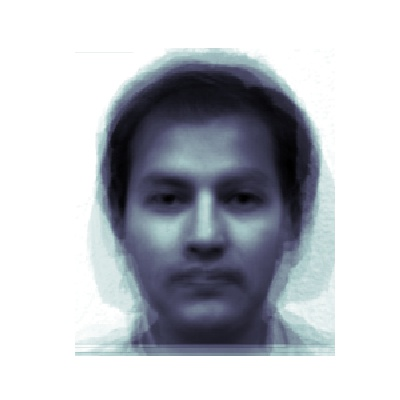
\includegraphics[width=0.4\textwidth]{./image/mean.jpg}

The mean face.

\newpage

\begin{figure}[htbp]
  \centering
  \subfigure[Eigen Faces 0]{
    \label{fig:ef0} %% label for first subfigure
    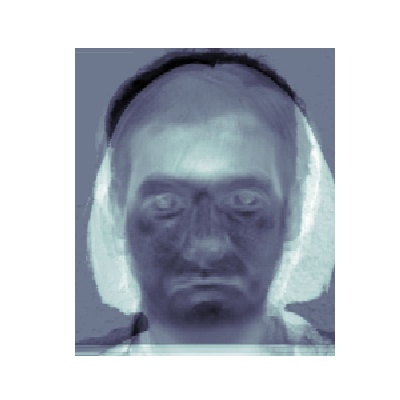
\includegraphics[width=0.2\textwidth]{./image/0.jpg}}
  \subfigure[Eigen Faces 1]{
    \label{fig:ef1} %% label for second subfigure
    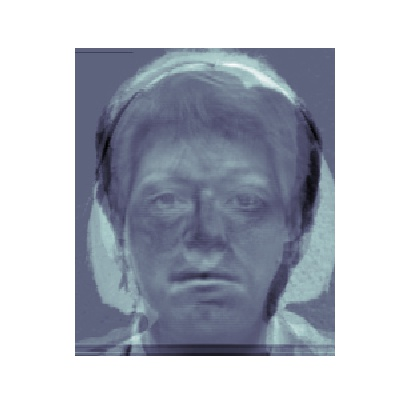
\includegraphics[width=0.2\textwidth]{./image/1.jpg}}
  \subfigure[Eigen Faces 2]{
    \label{fig:ef2} %% label for first subfigure
    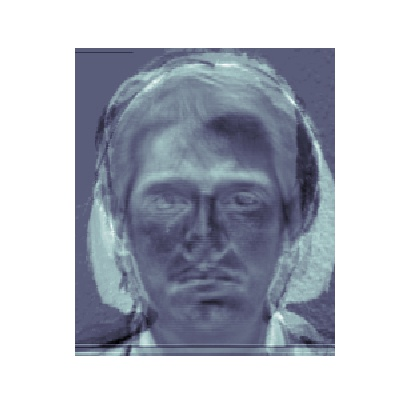
\includegraphics[width=0.2\textwidth]{./image/2.jpg}}
  \subfigure[Eigen Faces 3]{
    \label{fig:ef3} %% label for second subfigure
    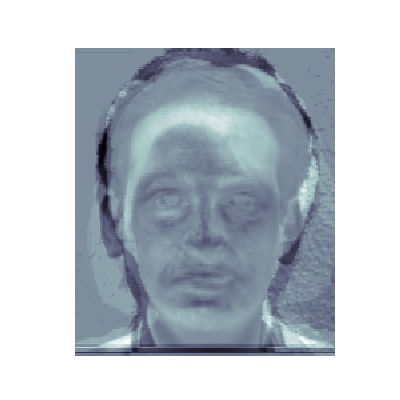
\includegraphics[width=0.2\textwidth]{./image/3.jpg}}
  \subfigure[Eigen Faces 0]{
    \label{fig:ef4} %% label for first subfigure
    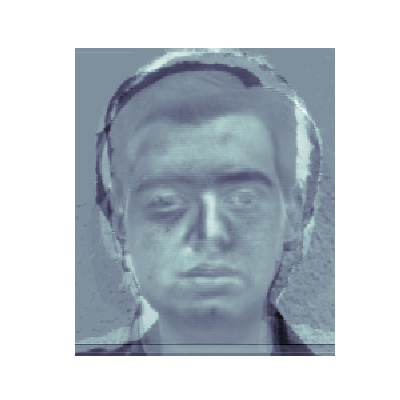
\includegraphics[width=0.2\textwidth]{./image/4.jpg}}
  \subfigure[Eigen Faces 1]{
    \label{fig:ef5} %% label for second subfigure
    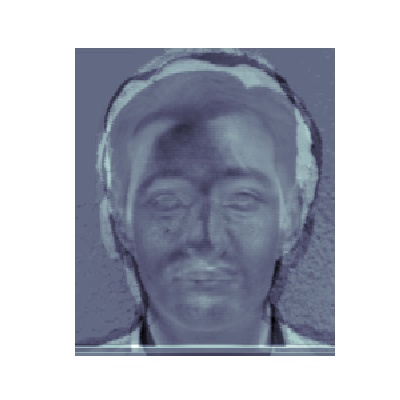
\includegraphics[width=0.2\textwidth]{./image/5.jpg}}
  \subfigure[Eigen Faces 2]{
    \label{fig:ef6} %% label for first subfigure
    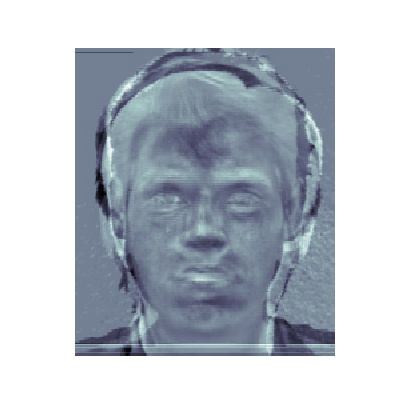
\includegraphics[width=0.2\textwidth]{./image/6.jpg}}
  \subfigure[Eigen Faces 3]{
    \label{fig:ef7} %% label for second subfigure
    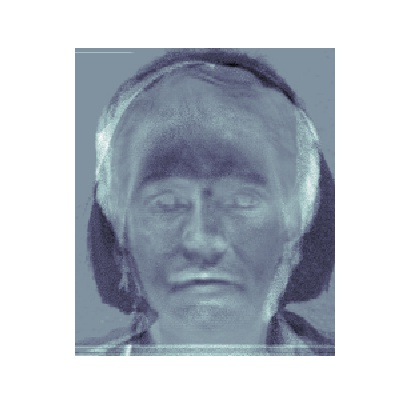
\includegraphics[width=0.2\textwidth]{./image/7.jpg}}
\caption{Eigen Faces}
  \label{fig:ef} %% label for entire figure
\end{figure}

The eigen space.

\begin{figure}[H]
  \centering
  \subfigure[Eigen Faces 0]{
    \label{fig:ef10} %% label for first subfigure
    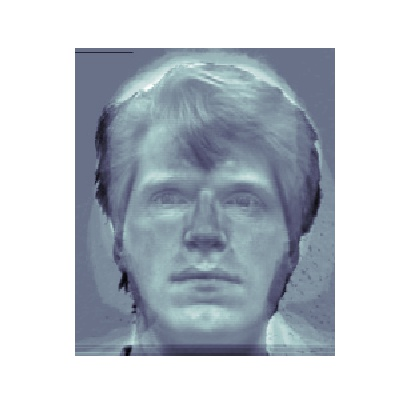
\includegraphics[width=0.2\textwidth]{./image/train/1.jpg}}
  \subfigure[Eigen Faces 1]{
    \label{fig:ef11} %% label for second subfigure
    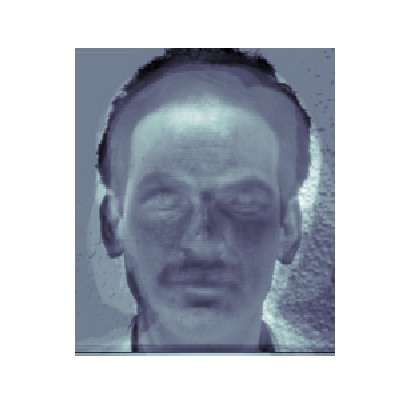
\includegraphics[width=0.2\textwidth]{./image/train/2.jpg}}
  \subfigure[Eigen Faces 2]{
    \label{fig:ef12} %% label for first subfigure
    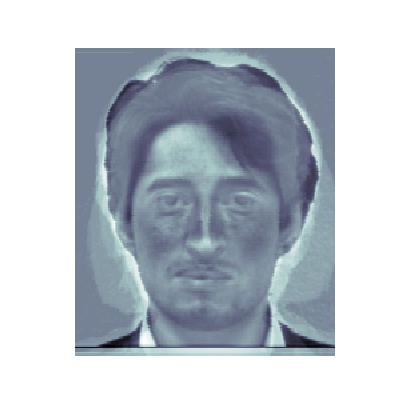
\includegraphics[width=0.2\textwidth]{./image/train/3.jpg}}
  \subfigure[Eigen Faces 3]{
    \label{fig:ef13} %% label for second subfigure
    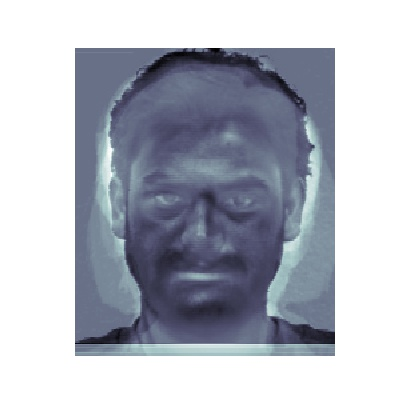
\includegraphics[width=0.2\textwidth]{./image/train/4.jpg}}
  \subfigure[Eigen Faces 0]{
    \label{fig:ef14} %% label for first subfigure
    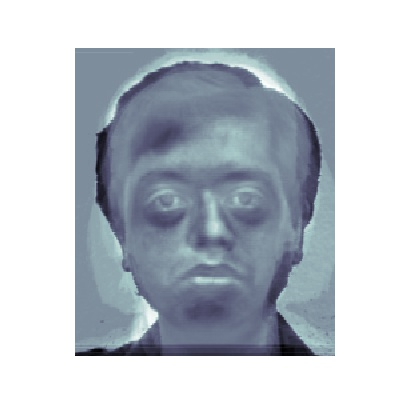
\includegraphics[width=0.2\textwidth]{./image/train/5.jpg}}
  \subfigure[Eigen Faces 1]{
    \label{fig:ef15} %% label for second subfigure
    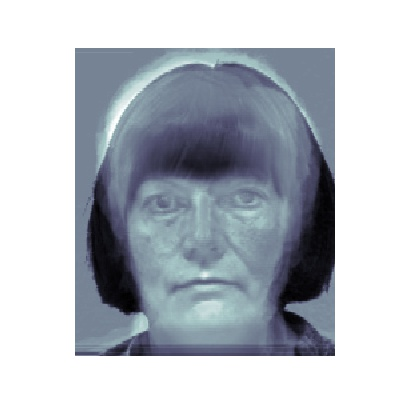
\includegraphics[width=0.2\textwidth]{./image/train/6.jpg}}
  \subfigure[Eigen Faces 2]{
    \label{fig:ef16} %% label for first subfigure
    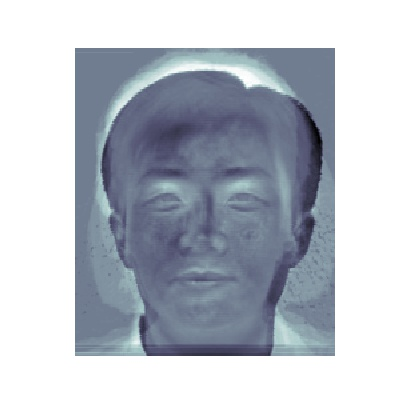
\includegraphics[width=0.2\textwidth]{./image/train/7.jpg}}
  \subfigure[Eigen Faces 3]{
    \label{fig:ef17} %% label for second subfigure
    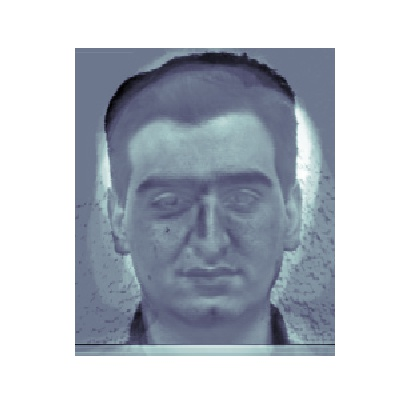
\includegraphics[width=0.2\textwidth]{./image/train/8.jpg}}
\caption{Train Face}
  \label{fig:ef} %% label for entire figure
\end{figure}

\newpage

\begin{figure}[htbp]
  \centering
  \subfigure[test image]{
    \label{fig:test:1.1} %% label for first subfigure
    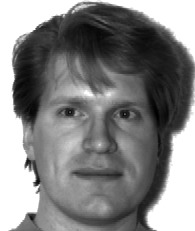
\includegraphics[width=0.2\textwidth]{./test_data/subject01_centerlight.jpg}}
  \subfigure[subtracting image]{
    \label{fig:sub:1.1} %% label for second subfigure
    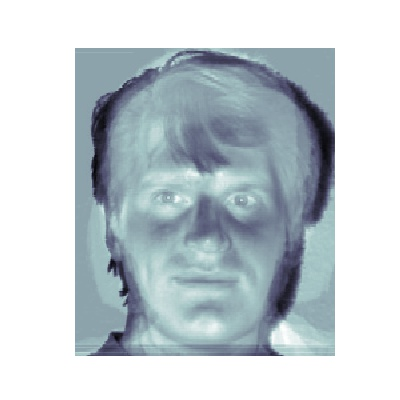
\includegraphics[width=0.2\textwidth]{./image/test/subject01_centerlight.jpg}}
  \subfigure[reconstructed image]{
    \label{fig:rec:1.1} %% label for second subfigure
    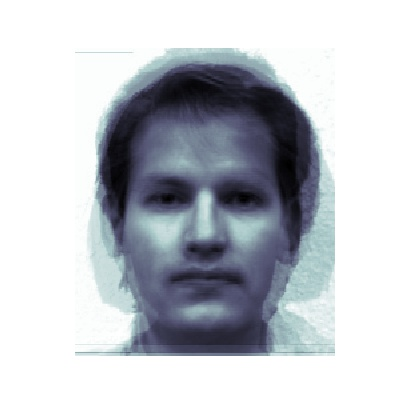
\includegraphics[width=0.2\textwidth]{./image/rec/subject01_centerlight.jpg}}
  \subfigure[result image]{
    \label{fig:result:1.1} %% label for second subfigure
    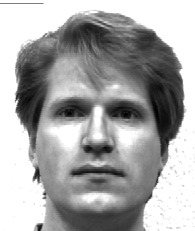
\includegraphics[width=0.2\textwidth]{./results/results_subject01_centerlight.jpg}}
\caption{Label 1}
  \label{fig:result 1} %% label for entire figure
\end{figure}

The distance from the projected test image to its nearest neighbor
is $188439677.034777$.

For the first face, if we use Euclidean Distance, it won't be detected correctly.
If we use Manhattan Distance, it will be detected correctly.

\begin{figure}[htbp]
  \centering
  \subfigure[test image]{
    \label{fig:subfig:1.2} %% label for first subfigure
    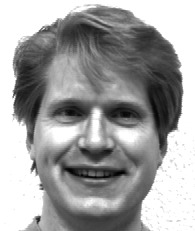
\includegraphics[width=0.2\textwidth]{./test_data/subject01_happy.jpg}}
  \subfigure[subtracting image]{
    \label{fig:subfig:1.2} %% label for first subfigure
    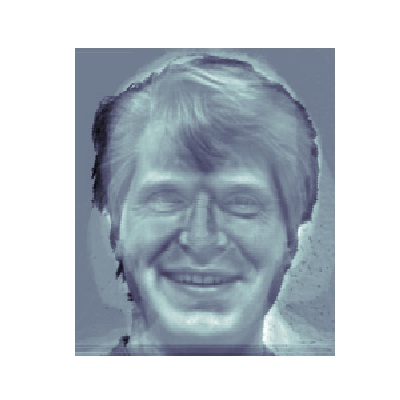
\includegraphics[width=0.2\textwidth]{./image/test/subject01_happy.jpg}}
  \subfigure[reconstructed image]{
    \label{fig:subfig:1.2} %% label for first subfigure
    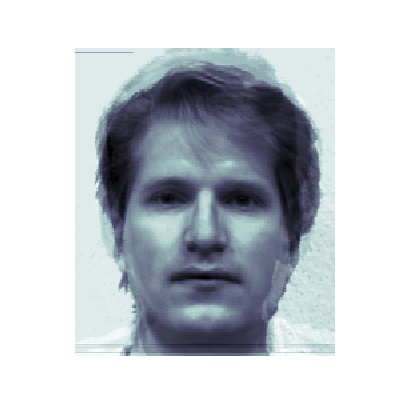
\includegraphics[width=0.2\textwidth]{./image/rec/subject01_happy.jpg}}
  \subfigure[result image]{
    \label{fig:subfig:1.2} %% label for second subfigure
    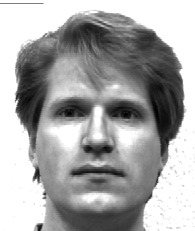
\includegraphics[width=0.2\textwidth]{./results/results_subject01_happy.jpg}}
\caption{Label 1}
  \label{fig:result 1} %% label for entire figure
\end{figure}

The distance from the projected test image to its nearest neighbor
is $106821588.638217$.

\begin{figure}[H]
  \centering
  \subfigure[test image]{
    \label{fig:subfig:1.3} %% label for first subfigure
    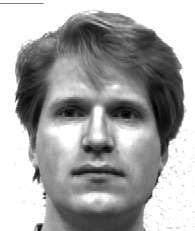
\includegraphics[width=0.2\textwidth]{./test_data/subject01_normal.jpg}}
  \subfigure[subtracting image]{
    \label{fig:subfig:1.3} %% label for first subfigure
    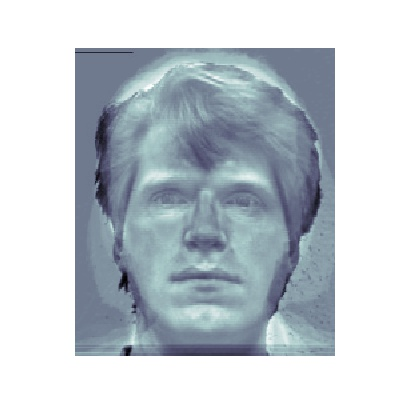
\includegraphics[width=0.2\textwidth]{./image/test/subject01_normal.jpg}}
  \subfigure[reconstructed image]{
    \label{fig:subfig:1.3} %% label for first subfigure
    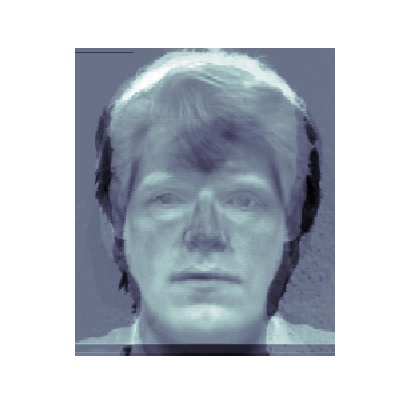
\includegraphics[width=0.2\textwidth]{./image/rec/subject01_normal.jpg}}
  \subfigure[result image]{
    \label{fig:subfig:1.3} %% label for second subfigure
    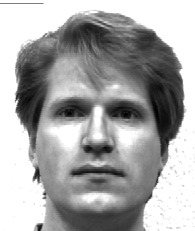
\includegraphics[width=0.2\textwidth]{./results/results_subject01_normal.jpg}}
\caption{Label 1}
  \label{fig:result 1} %% label for entire figure
\end{figure}

The distance from the projected test image to its nearest neighbor
is $0.0$.\\

\newpage

\begin{figure}[htbp]
  \centering
  \subfigure[test image]{
    \label{fig:subfig:2.3} %% label for first subfigure
    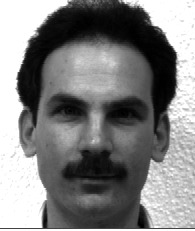
\includegraphics[width=0.2\textwidth]{./test_data/subject02_normal.jpg}}
  \subfigure[subtracting image]{
    \label{fig:subfig:2.3} %% label for first subfigure
    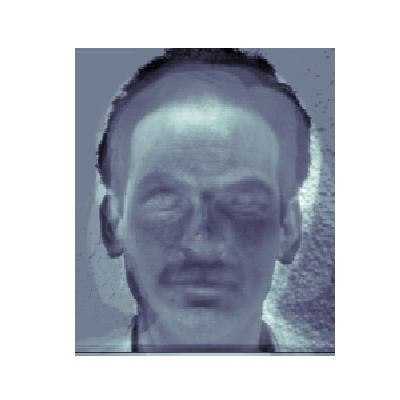
\includegraphics[width=0.2\textwidth]{./image/test/subject02_normal.jpg}}
  \subfigure[reconstructed image]{
    \label{fig:subfig:2.3} %% label for first subfigure
    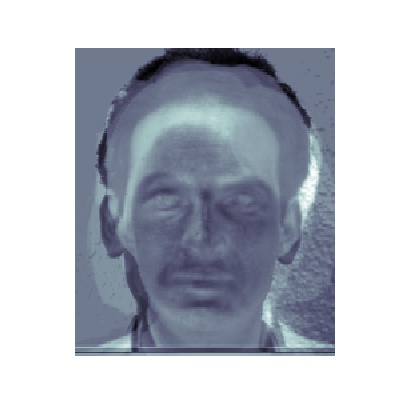
\includegraphics[width=0.2\textwidth]{./image/rec/subject02_normal.jpg}}
  \subfigure[result image]{
    \label{fig:subfig:2.3} %% label for second subfigure
    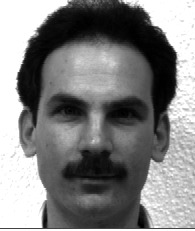
\includegraphics[width=0.2\textwidth]{./results/results_subject02_normal.jpg}}
\caption{Label 2}
  \label{fig:result 2} %% label for entire figure
\end{figure}

The distance from the projected test image to its nearest neighbor
is $0.0$.\\

For 2nd face, the test image is also the train image, it should be correctly.


\begin{figure}[htbp]
  \centering
  \subfigure[test image]{
    \label{fig:subfig:3.1} %% label for first subfigure
    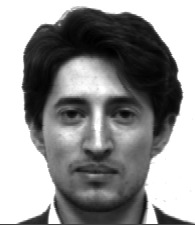
\includegraphics[width=0.2\textwidth]{./test_data/subject03_normal.jpg}}
  \subfigure[subtracting image]{
    \label{fig:subfig:3.2} %% label for first subfigure
    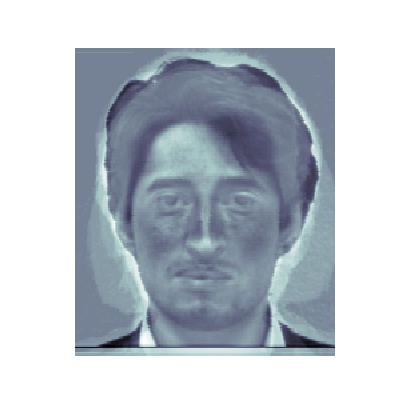
\includegraphics[width=0.2\textwidth]{./image/test/subject03_normal.jpg}}
  \subfigure[reconstructed image]{
    \label{fig:subfig:3.3} %% label for first subfigure
    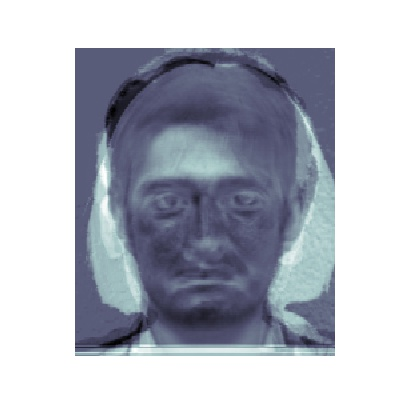
\includegraphics[width=0.2\textwidth]{./image/rec/subject03_normal.jpg}}
  \subfigure[result image]{
    \label{fig:subfig:3.4} %% label for second subfigure
    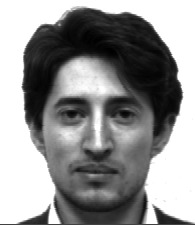
\includegraphics[width=0.2\textwidth]{./results/results_subject03_normal.jpg}}
\caption{Label 3}
  \label{fig:result 3} %% label for entire figure
\end{figure}

The distance from the projected test image to its nearest neighbor
is $0.0$.\\

For the 3rd face, the test image is also the train image, it should be correctly.

\newpage

\begin{figure}[htbp]
  \centering
  \subfigure[test image]{
    \label{fig:test:7.1} %% label for first subfigure
    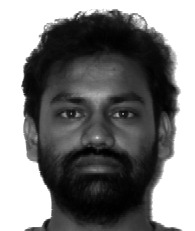
\includegraphics[width=0.2\textwidth]{./test_data/subject07_centerlight.jpg}}
  \subfigure[subtracting image]{
    \label{fig:sub:7.1} %% label for second subfigure
    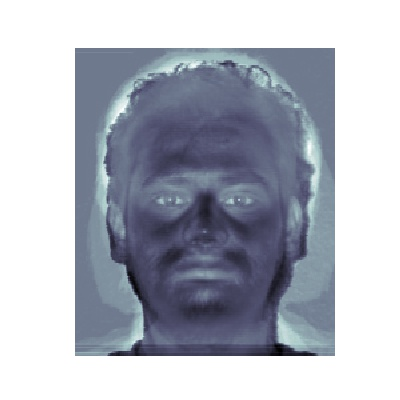
\includegraphics[width=0.2\textwidth]{./image/test/subject07_centerlight.jpg}}
  \subfigure[reconstructed image]{
    \label{fig:rec:7.1} %% label for second subfigure
    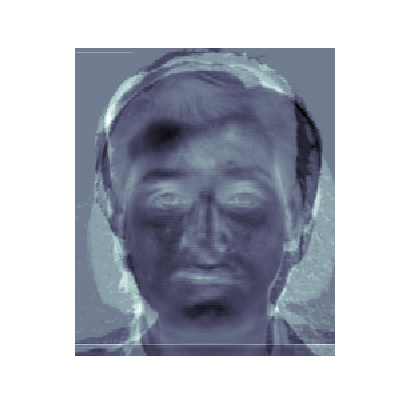
\includegraphics[width=0.2\textwidth]{./image/rec/subject07_centerlight.jpg}}
\caption{Label 7}
  \label{fig:result 7} %% label for entire figure
\end{figure}

This image is detected as non-face.

\begin{figure}[htbp]
  \centering
  \subfigure[test image]{
    \label{fig:subfig:7.2} %% label for first subfigure
    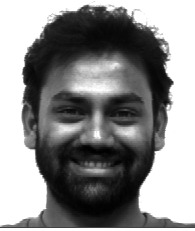
\includegraphics[width=0.2\textwidth]{./test_data/subject07_happy.jpg}}
  \subfigure[subtracting image]{
    \label{fig:subfig:7.2} %% label for first subfigure
    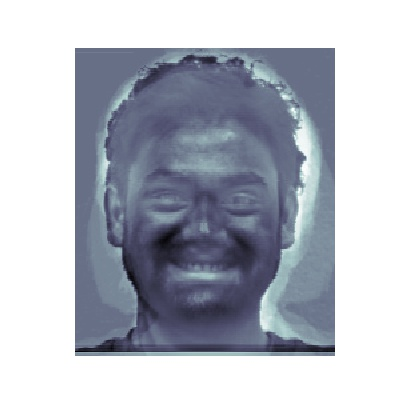
\includegraphics[width=0.2\textwidth]{./image/test/subject07_happy.jpg}}
  \subfigure[reconstructed image]{
    \label{fig:subfig:7.2} %% label for first subfigure
    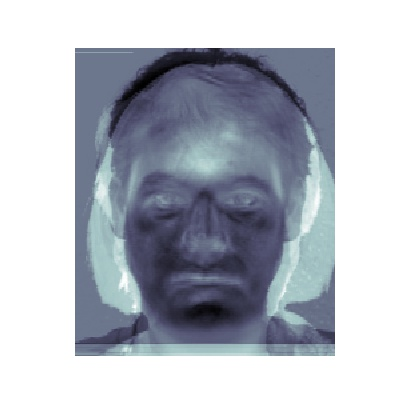
\includegraphics[width=0.2\textwidth]{./image/rec/subject07_happy.jpg}}
  \subfigure[result image]{
    \label{fig:subfig:7.2} %% label for second subfigure
    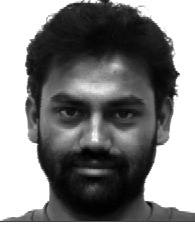
\includegraphics[width=0.2\textwidth]{./results/results_subject07_happy.jpg}}
\caption{Label 7}
  \label{fig:result 7} %% label for entire figure
\end{figure}

The distance from the projected test image to its nearest neighbor
is $173336241.992190$.

\begin{figure}[H]
  \centering
  \subfigure[test image]{
    \label{fig:subfig:7.3} %% label for first subfigure
    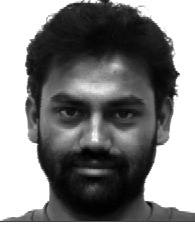
\includegraphics[width=0.2\textwidth]{./test_data/subject07_normal.jpg}}
  \subfigure[subtracting image]{
    \label{fig:subfig:7.3} %% label for first subfigure
    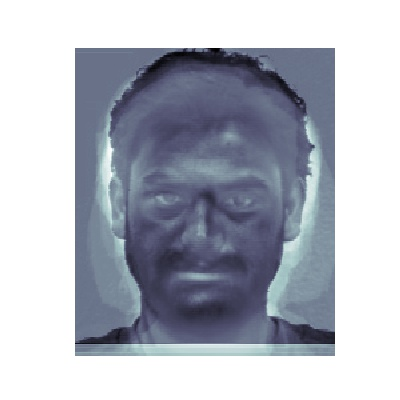
\includegraphics[width=0.2\textwidth]{./image/test/subject07_normal.jpg}}
  \subfigure[reconstructed image]{
    \label{fig:subfig:7.3} %% label for first subfigure
    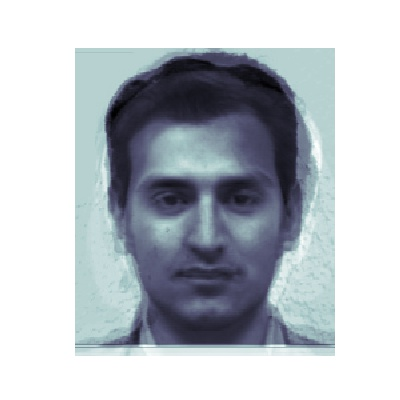
\includegraphics[width=0.2\textwidth]{./image/rec/subject07_normal.jpg}}
  \subfigure[result image]{
    \label{fig:subfig:7.3} %% label for second subfigure
    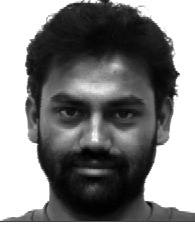
\includegraphics[width=0.2\textwidth]{./results/results_subject07_normal.jpg}}
\caption{Label 7}
  \label{fig:result 7} %% label for entire figure
\end{figure}

The distance from the projected test image to its nearest neighbor
is $0.0$.\\

\newpage

\begin{figure}[htbp]
  \centering
  \subfigure[test image]{
    \label{fig:subfig:10.3} %% label for first subfigure
    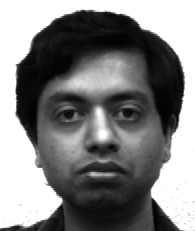
\includegraphics[width=0.2\textwidth]{./test_data/subject10_normal.jpg}}
  \subfigure[subtracting image]{
    \label{fig:subfig:10.3} %% label for first subfigure
    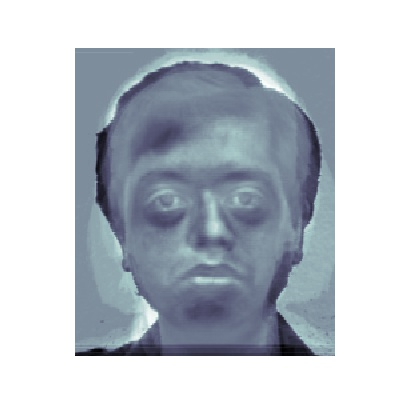
\includegraphics[width=0.2\textwidth]{./image/test/subject10_normal.jpg}}
  \subfigure[reconstructed image]{
    \label{fig:subfig:10.3} %% label for first subfigure
    \includegraphics[width=0.2\textwidth]{./image/rec/subject10_normal.jpg}}
  \subfigure[result image]{
    \label{fig:subfig:10.3} %% label for second subfigure
    \includegraphics[width=0.2\textwidth]{./results/results_subject10_normal.jpg}}
\caption{Label 10}
  \label{fig:result 10} %% label for entire figure
\end{figure}

The distance from the projected test image to its nearest neighbor
is $0.0$.\\

The test image is also the train image, it should be correctly.

\newpage

\begin{figure}[htbp]
  \centering
  \subfigure[test image]{
    \label{fig:test:11.1} %% label for first subfigure
    \includegraphics[width=0.2\textwidth]{./test_data/subject11_centerlight.jpg}}
  \subfigure[subtracting image]{
    \label{fig:sub:11.1} %% label for second subfigure
    \includegraphics[width=0.2\textwidth]{./image/test/subject11_centerlight.jpg}}
  \subfigure[reconstructed image]{
    \label{fig:rec:11.1} %% label for second subfigure
    \includegraphics[width=0.2\textwidth]{./image/rec/subject11_centerlight.jpg}}
  \subfigure[result image]{
    \label{fig:result:11.1} %% label for second subfigure
    \includegraphics[width=0.2\textwidth]{./results/results_subject11_centerlight.jpg}}
\caption{Label 11}
  \label{fig:result 11} %% label for entire figure
\end{figure}

The distance from the projected test image to its nearest neighbor
is $190962100.776104$.

\begin{figure}[htbp]
  \centering
  \subfigure[test image]{
    \label{fig:subfig:11.2} %% label for first subfigure
    \includegraphics[width=0.2\textwidth]{./test_data/subject11_happy.jpg}}
  \subfigure[subtracting image]{
    \label{fig:subfig:11.2} %% label for first subfigure
    \includegraphics[width=0.2\textwidth]{./image/test/subject11_happy.jpg}}
  \subfigure[reconstructed image]{
    \label{fig:subfig:11.2} %% label for first subfigure
    \includegraphics[width=0.2\textwidth]{./image/rec/subject11_happy.jpg}}
  \subfigure[result image]{
    \label{fig:subfig:11.2} %% label for second subfigure
    \includegraphics[width=0.2\textwidth]{./results/results_subject11_happy.jpg}}
\caption{Label 11}
  \label{fig:result 11} %% label for entire figure
\end{figure}

The distance from the projected test image to its nearest neighbor
is $37711066.350580$.

\begin{figure}[H]
  \centering
  \subfigure[test image]{
    \label{fig:subfig:11.3} %% label for first subfigure
    \includegraphics[width=0.2\textwidth]{./test_data/subject11_normal.jpg}}
  \subfigure[subtracting image]{
    \label{fig:subfig:11.3} %% label for first subfigure
    \includegraphics[width=0.2\textwidth]{./image/test/subject11_normal.jpg}}
  \subfigure[reconstructed image]{
    \label{fig:subfig:11.3} %% label for first subfigure
    \includegraphics[width=0.2\textwidth]{./image/rec/subject11_normal.jpg}}
  \subfigure[result image]{
    \label{fig:subfig:11.3} %% label for second subfigure
    \includegraphics[width=0.2\textwidth]{./results/results_subject11_normal.jpg}}
\caption{Label 11}
  \label{fig:result 11} %% label for entire figure
\end{figure}

The distance from the projected test image to its nearest neighbor
is $0.0$.\\

For the 11th face, all three test image are detected correctly.

\newpage

\begin{figure}[htbp]
  \centering
  \subfigure[test image]{
    \label{fig:subfig:12.3} %% label for first subfigure
    \includegraphics[width=0.2\textwidth]{./test_data/subject12_normal.jpg}}
  \subfigure[subtracting image]{
    \label{fig:subfig:12.3} %% label for first subfigure
    \includegraphics[width=0.2\textwidth]{./image/test/subject12_normal.jpg}}
  \subfigure[reconstructed image]{
    \label{fig:subfig:12.3} %% label for first subfigure
    \includegraphics[width=0.2\textwidth]{./image/rec/subject12_normal.jpg}}
  \subfigure[result image]{
    \label{fig:subfig:12.3} %% label for second subfigure
    \includegraphics[width=0.2\textwidth]{./results/results_subject12_normal.jpg}}
\caption{Label 12}
  \label{fig:result 12} %% label for entire figure
\end{figure}

The distance from the projected test image to its nearest neighbor
is $172771700.658602$.

\begin{figure}[htbp]
  \centering
  \subfigure[test image]{
    \label{fig:test:14.1} %% label for first subfigure
    \includegraphics[width=0.2\textwidth]{./test_data/subject14_sad.jpg}}
  \subfigure[subtracting image]{
    \label{fig:sub:14.1} %% label for second subfigure
    \includegraphics[width=0.2\textwidth]{./image/test/subject14_sad.jpg}}
  \subfigure[reconstructed image]{
    \label{fig:rec:14.1} %% label for second subfigure
    \includegraphics[width=0.2\textwidth]{./image/rec/subject14_sad.jpg}}
  \subfigure[result image]{
    \label{fig:result:14.1} %% label for second subfigure
    \includegraphics[width=0.2\textwidth]{./results/results_subject14_sad.jpg}}
\caption{Label 14}
  \label{fig:result 14} %% label for entire figure
\end{figure}

The distance from the projected test image to its nearest neighbor
is $38834390.761937$.

\begin{figure}[htbp]
  \centering
  \subfigure[test image]{
    \label{fig:subfig:14.2} %% label for first subfigure
    \includegraphics[width=0.2\textwidth]{./test_data/subject14_happy.jpg}}
  \subfigure[subtracting image]{
    \label{fig:subfig:14.2} %% label for first subfigure
    \includegraphics[width=0.2\textwidth]{./image/test/subject14_happy.jpg}}
  \subfigure[reconstructed image]{
    \label{fig:subfig:14.2} %% label for first subfigure
    \includegraphics[width=0.2\textwidth]{./image/rec/subject14_happy.jpg}}
  \subfigure[result image]{
    \label{fig:subfig:14.2} %% label for second subfigure
    \includegraphics[width=0.2\textwidth]{./results/results_subject14_happy.jpg}}
\caption{Label 14}
  \label{fig:result 14} %% label for entire figure
\end{figure}

The distance from the projected test image to its nearest neighbor
is $44587580.401787$.

\begin{figure}[H]
  \centering
  \subfigure[test image]{
    \label{fig:subfig:14.3} %% label for first subfigure
    \includegraphics[width=0.2\textwidth]{./test_data/subject14_normal.jpg}}
  \subfigure[subtracting image]{
    \label{fig:subfig:14.3} %% label for first subfigure
    \includegraphics[width=0.2\textwidth]{./image/test/subject14_normal.jpg}}
  \subfigure[reconstructed image]{
    \label{fig:subfig:14.3} %% label for first subfigure
    \includegraphics[width=0.2\textwidth]{./image/rec/subject14_normal.jpg}}
  \subfigure[result image]{
    \label{fig:subfig:14.3} %% label for second subfigure
    \includegraphics[width=0.2\textwidth]{./results/results_subject14_normal.jpg}}
\caption{Label 14}
  \label{fig:result 14} %% label for entire figure
\end{figure}

The distance from the projected test image to its nearest neighbor
is $0.0$.\\

For the 14th face, all three test image are detected correctly.

\newpage

\begin{figure}[htbp]
  \centering
  \subfigure[test image]{
    \label{fig:subfig:15.3} %% label for first subfigure
    \includegraphics[width=0.2\textwidth]{./test_data/subject15_normal.jpg}}
  \subfigure[subtracting image]{
    \label{fig:subfig:15.3} %% label for first subfigure
    \includegraphics[width=0.2\textwidth]{./image/test/subject15_normal.jpg}}
  \subfigure[reconstructed image]{
    \label{fig:subfig:15.3} %% label for first subfigure
    \includegraphics[width=0.2\textwidth]{./image/rec/subject15_normal.jpg}}
  \subfigure[result image]{
    \label{fig:subfig:15.3} %% label for second subfigure
    \includegraphics[width=0.2\textwidth]{./results/results_subject15_normal.jpg}}
\caption{Label 15}
  \label{fig:result 15} %% label for entire figure
\end{figure}

The distance from the projected test image to its nearest neighbor
is $0.0$.\\

For the 15th face, the test image is also the train image, it should be correctly.

\begin{figure}[htbp]
  \centering
  \subfigure[test image]{
    \label{fig:subfig:0.1} %% label for first subfigure
    \includegraphics[width=0.2\textwidth]{./test_data/apple1_gray.jpg}}
  \subfigure[subtracting image]{
    \label{fig:subfig:0.3} %% label for first subfigure
    \includegraphics[width=0.2\textwidth]{./image/test/apple1_gray.jpg}}
  \subfigure[reconstructed image]{
    \label{fig:subfig:0.3} %% label for first subfigure
    \includegraphics[width=0.2\textwidth]{./image/rec/apple1_gray.jpg}}
  \caption{Non-face}
  \label{fig:result 0.1} %% label for entire figure
\end{figure}

This image is detected as non-face.

\newpage

\titleformat{\chapter}[display]
          {\normalfont\Large\bfseries}{Appendix~\Alph{chapter}}{11pt}{\Large}

\begin{appendices}
\renewcommand{\thechapter}{\Alph{chapter}.}
  \chapter{Source Code}
  \inputpython{../eigenfaces.py}{0}{299}
\end{appendices}


\clearpage

\backmatter

\end{document}
